\subsection{凸函数的定义}

定义 1. 我们说，有限数值函数 \(f\) （定义在区间 \(\mathrm{I} \subset \mathbf{R}\) 上的）在 \(\mathrm{I}\) 上是凸的，如果不论点 \(x, x'\) （\(\mathrm{I}\) 中的，\((x < x')\) ）如何，每一点 \(\mathrm{M}_z\) （属于图像 \(\mathrm{G}\) ，即 \(f\) 的图像，且满足 \(x \leqslant z \leqslant x'\) 的）都位于线段 \(\mathrm{M}_x\mathrm{M}_{x'}\) 之下（或者，等价地，如果此线段的每一点都位于 \(\mathrm{G}\) 之上）（fig.~2）。

\pandocbounded{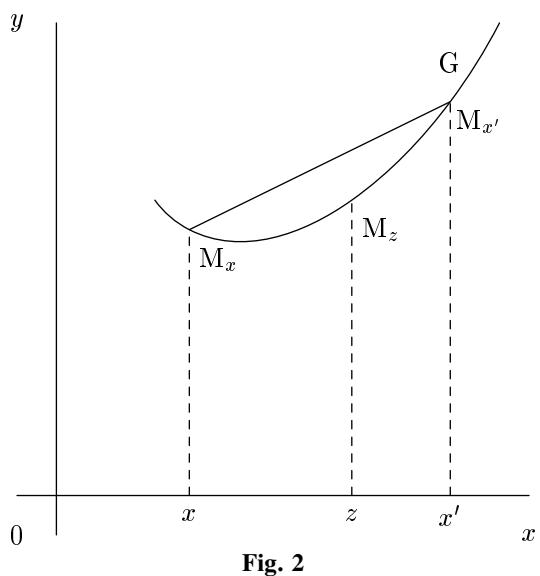
\includegraphics[keepaspectratio]{images/part001_0967d261.jpg}}

考虑到线段的参数表示（Gen.~Top., VI, p.~35），f 在 I 上凸的条件是不等式

\[
f (\lambda x + (1 - \lambda) x ^ {\prime}) \leqslant \lambda f (x) + (1 - \lambda) f (x ^ {\prime})\tag{1}
\]

对 I 的每一对点 \((x, x')\) 及每个 \(\lambda \in [0, 1]\) 成立。

定义 1 等价于：\(\mathbf{R}^2\) 中位于图像 \(G\) （即 \(f\) 的图像）上方的点所成的集是凸的。事实上，这一条件显然足以使 \(f\) 在 I 上凸；它也是必要的，因为若 \(f\) 在 I 上凸，且 \((x,y)\) 、\((x',y')\) 是位于 \(G\) 上方的两点，则有 \(y \geqslant f(x)\) ，\(y' \geqslant f(x')\) ，由此，对 \(0 \leqslant \lambda \leqslant 1\) ，

\[
\lambda y + (1 - \lambda) y ^ {\prime} \geqslant \lambda f (x) + (1 - \lambda) f \left(x ^ {\prime}\right) \geqslant f (\lambda x + (1 - \lambda) x ^ {\prime})
\]

（由 (1)），这表明以 \((x, y)\) 与 \((x', y')\) 为端点的线段的每一点都位于 G 上方。

注. 同样可以看出，严格位于 G 上方的点所成的集是凸的。反之，若此集是凸的，则有

\[
\lambda y + (1 - \lambda) y ^ {\prime} > f (\lambda x + (1 - \lambda) x ^ {\prime})
\]

对 \(0 \leqslant \lambda \leqslant 1\) 及 \(y > f(x)\) 、\(y' > f(x')\) 成立；在此公式中让 \(y\) 趋于 \(f(x)\) 、\(y'\) 趋于 \(f(x')\) ，便得出 \(f\) 是凸的。

例。1) 每个（实）仿射线性函数 \(ax + b\) 在 \(\mathbf{R}\) 上都是凸的。

\begin{enumerate}
\def\labelenumi{\arabic{enumi})}
\setcounter{enumi}{1}
\tightlist
\item
  函数 \(x^{2}\) 在 \(\mathbf{R}\) 上是凸的，因为有
\end{enumerate}

\[
\lambda x ^ {2} + (1 - \lambda) x ^ {\prime 2} - \left(\lambda x + (1 - \lambda) x ^ {\prime}\right) ^ {2} = \lambda (1 - \lambda) (x - x ^ {\prime}) ^ {2} \geqslant 0
\]

对 \(0 \leqslant \lambda \leqslant 1\) 。

\begin{enumerate}
\def\labelenumi{\arabic{enumi})}
\setcounter{enumi}{2}
\tightlist
\item
  函数 \(|x|\) 在 \(\mathbf{R}\) 上是凸的，因为
\end{enumerate}

\[
\left| \lambda x + (1 - \lambda) x ^ {\prime} \right| \leqslant \lambda | x | + (1 - \lambda) \left| x ^ {\prime} \right|
\]

对 \(0 \leqslant \lambda \leqslant 1\) 。

显然，若 \(f\) 在 \(\mathbf{I}\) 上凸，则它在任何区间 \(\mathbf{J} \subset \mathbf{I}\) 上的限制在 \(\mathbf{J}\) 上凸。

设 \(f\) 是 \(I\) 上的凸函数，\(x, x'\) 是 \(I\) 中两点，满足 \(x < x'\) ；若 \(z \in I\) 在 \([x, x']\) 之外，则 \(M_z\) 位于直线 \(D\) （联结 \(M_x\) 与 \(M_{x'}\) 的）上方；这是引理的直接推论。

由此推出：若 z 是满足 \(x < z < x'\) 的点且 \(M_{z}\) 位于线段 \(M_{x}M_{x'}\) 上，则对任何别的点 \(z'\) （满足 \(x < z' < x'\) 的），点 \(M_{z'}\) 也位于线段 \(M_{x}M_{x'}\) 上，因为由上所述 \(M_{z'}\) 同时位于此线段的上方和下方；换句话说，此时 f 在 \([x, x']\) 上等于一个仿射线性函数。

定义 2. 我们说，有限实函数 \(f\) （定义在区间 \(\mathbf{I} \subset \mathbf{R}\) 上的）在 \(\mathbf{I}\) 上是严格凸的，如果对任意点 \(x, x'\) （\(\mathbf{I}\) 中的， \(x < x'\) ），每一点 \(\mathbf{M}_z\) （属于图像 \(\mathbf{G}\) ，即 \(f\) 的图像，且满足 \(x < z < x'\) 的）都严格位于线段 \(\mathbf{M}_x\mathbf{M}_{x'}\) 之下（或者，等价地，如果此线段的每一点除端点外都严格位于 \(\mathbf{G}\) 之上）。

换句话说，必须有不等式

\[
f (\lambda x + (1 - \lambda) x ^ {\prime}) <   \lambda f (x) + (1 - \lambda) f (x ^ {\prime})\tag{2}
\]

对 I 的每一对不同的点 \((x, x')\) 及每个 \(\lambda\) （满足 \(0 < \lambda < 1\) 的）成立。

定义 2 之前的那些说明表明：为使凸函数 f 在 I 上严格凸，当且仅当不存在包含在 I 中的（不退化为一点的）区间使得 f 在其上的限制是仿射线性的。

在上面的例子中，第一个和第三个不是严格凸的；另一方面，\(x^2\) 在 \(\mathbf{R}\) 上严格凸；类似的计算表明 \(1 / x\) 在 \(]0, +\infty[\) 上严格凸。

命题 1. 设 \(f\) 是有限实函数，在区间 \(\mathbf{I} \subset \mathbf{R}\) 上凸（相应地，严格凸）。对每一家族 \((x_i)_{1 \leqslant i \leqslant p}\) （由 \(p \geqslant 2\) 个属于 \(\mathbf{I}\) 的不同的点组成），及每一家族 \((\lambda_i)_{1 \leqslant i \leqslant p}\) （由 \(p\) 个实数组成，满足 \(0 < \lambda_i < 1\) 且 \(\sum_{i=1}^{p} \lambda_i = 1\) ），我们有

\[
f \left(\sum_ {i = 1} ^ {p} \lambda_ {i} x _ {i}\right) \leqslant \sum_ {i = 1} ^ {p} \lambda_ {i} f (x _ {i})\tag{3}
\]

（相应地，

\[
f \left(\sum_ {i = 1} ^ {p} \lambda_ {i} x _ {i}\right) <   \sum_ {i = 1} ^ {p} \lambda_ {i} f (x _ {i})).\tag{4}
\]

由于该命题（就凸函数而言）在 \(p = 2\) 时归结为不等式 (1)，我们对 \(p > 2\) 用归纳法论证。数 \(\mu = \sum_{i=1}^{p-1} \lambda_i\) 为 \(> 0\) ；立即可以看出，若 \(a\) 与 \(b\) 是诸 \(x_i\) 中最小者和最大者，则 \(a \leqslant \sum_{i=1}^{p-1} \lambda_i x_i / \sum_{i=1}^{p-1} \lambda_i \leqslant b\) ；换句话说，点 \(x = \frac{1}{\mu} \sum_{i=1}^{p-1} \lambda_i x_i\) 属于 I，且归纳假设蕴含 \(\mu f(x) \leqslant \sum_{i=1}^{p-1} \lambda_i f(x_i)\) ；此外，由 (1) 我们有

\[
f \left(\sum_ {i = 1} ^ {p} \lambda_ {i} x _ {i}\right) = f (\mu x + (1 - \mu) x _ {p}) \leqslant \mu f (x) + (1 - \mu) f (x _ {p}) \leqslant \sum_ {i = 1} ^ {p} \lambda_ {i} f (x _ {i}).
\]

对严格凸函数，从不等式 (2) 出发，同样论证。

我们说有限实函数 \(f\) 在 I 上是凹的（相应地，严格凹的），如果 \(-f\) 在 I 上是凸的（相应地，严格凸的）。这等价于说，对 I 的每一对不同的点 \((x, x')\) 及每个 \(\lambda\) （满足 \(0 < \lambda < 1\) 的），有

\[
f (\lambda x + (1 - \lambda) x ^ {\prime}) \geqslant \lambda f (x) + (1 - \lambda) f (x ^ {\prime})
\]

\[
(\text { resp. } f (\lambda x + (1 - \lambda) x ^ {\prime}) > \lambda f (x) + (1 - \lambda) f (x ^ {\prime})).
\]

